\documentclass{article}

% Language setting
% Replace `english' with e.g. `spanish' to change the document language
\usepackage[english]{babel}
\usepackage{{booktabs}}
\usepackage{rotating}
\usepackage{float}
\usepackage{multirow}
\usepackage{multicol}


% Set page size and margins
% Replace `letterpaper' with `a4paper' for UK/EU standard size
\usepackage[letterpaper,top=2cm,bottom=2cm,left=3cm,right=3cm,marginparwidth=1.75cm]{geometry}

% Useful packages
\usepackage{amsmath}
\usepackage{graphicx}
\usepackage[colorlinks=true, allcolors=blue]{hyperref}


\title{ISyE 6740 Tumor Detection}
\author{Paul Telford, Hannah Pavlovich}

\begin{document}
\maketitle

\begin{abstract}
Your abstract.
\end{abstract}

\tableofcontents

\section{Introduction}

In medicine, a brain \textbf{MRI (magnetic resonance imaging) scan} is a painless test that produces very clear images of the structures inside a patient's head — mainly, the brain. Healthcare providers use brain \textbf{MRIs} to evaluate, diagnose and monitor several different medical conditions that affect the brain or other structures in the head. Currently, \textbf{MRI} is the most sensitive imaging test for the brain. To enhance image quality, a patient's brain is often injected with a \textbf{*contrast agent*} like \textbf{gadolinium;} a rare earth metal that alters the magnetic properties of nearby water molecules. This improves the \textbf{sensitivity} and \textbf{specificity} of the diagnostic images. The contrast material enhances the visibility of \textbf{tumors, inflammation, blood vessels, etc.}

In this project, we'll investigate the performance of some common \textbf{classification techniques} with features based on \textbf{first and second order statistics} for the detection of \textbf{brain tumors}using a data set comprised of features extracted from \textbf{MRI} images. The performance will be evaluated in terms of \textbf{sensitivity, specificity,} and \textbf{accuracy.}

\section{Description of Data}\label{description-data}

The dataset is taken from kaggle: \textit{Brain Tumor: Extracted features for brain tumor}\cite{kaggle-set}, which includes data from 1,644 \textbf{MRI} image scans. The .csv data file consists of five first-order (textural) feature columns, eight second-order feature columns, and the class (target) column.

It is important to note at this juncture that we did not pre-process the raw \textbf{MRI} images ourselves. This process would typically involve the following steps:
\begin{enumerate}
    \item \textbf{Grayscale conversion -} RGB images contain unnecessary information that requires a lot of storage space
    \item \textbf{Filtering -} for elimination of common noises like salt and pepper and speckle in grayscale images by applying filtering techniques like Gaussian, mean, and median filter.
    \item \textbf{Feature Extraction -} shortening the number of resources needed to define a big group of data correctly. This is necessary because analysis of a huge number of variables requires more memory and computation time. The features that we are going to use for this exercise are typically extracted by way of a \textbf{Gray Level Co-occurrence Matrix (GLCM).} A \textbf{co-occurrence matrix} or \textbf{co-occurrence distribution} is defined over an image to be the distribution of co-occurrence values at a given offset. Meaning, values in the matrix represent the distance and angular spatial relationship over an image sub-region of specific size. Moreover, The \textbf{GLCM} calculates how often a pixel with gray-level (grayscale intensity or tone) value $i$ occurs either horizontally, vertically, or diagonally to adjacent pixels with the value $j$. Once the \textbf{GLCM} is created, several statistics similar to the ones we'll use for this exercise can be derived using different formulas.
\end{enumerate}

\subsection{First-Order Features}
Below is a description of the first-order feature columns contained in the raw data set.

\begin{table}[H]
    \centering
    \begin{tabular}{lrrrrrrrr}
    \toprule
     & Mean & Variance & Standard Deviation & Skewness & Kurtosis \\
    \midrule
    count & 3762.0000 & 3762.0000 & 3762.0000 & 3762.0000 & 3762.0000 \\
    mean & 9.4889 & 711.1011 & 25.1823 & 4.1027 & 24.3891 \\
    std & 5.7280 & 467.4669 & 8.7735 & 2.5609 & 56.4347 \\
    min & 0.0787 & 3.1456 & 1.7736 & 1.8860 & 3.9424 \\
    25\% & 4.9824 & 363.2255 & 19.0585 & 2.6202 & 7.2529 \\
    50\% & 8.4775 & 622.5804 & 24.9516 & 3.4222 & 12.3591 \\
    75\% & 13.2127 & 966.9543 & 31.0959 & 4.6517 & 22.6403 \\
    max & 33.2400 & 2910.5819 & 53.9498 & 36.9313 & 1371.6401 \\
    \bottomrule
    \end{tabular}
    \caption{Description of First Order Features}
    \label{fo-features}
\end{table}

\begin{itemize}
    \item  \textbf{Variance} is a measure of the histogram width which represents the deviation of gray levels from the mean. 
    \item \textbf{Skewness} is a measure of the degree of histogram asymmetry around the mean, and 
    \item \textbf{Kurtosis} is a measure of the histogram sharpness and is given by:
\[
Kurtosis\ = \frac{1}{mn}\sum\limits_{i=1}^m\sum\limits_{j=1}^n\left\{\left[\frac{P_{i,j}-\sigma}{\sigma}\right]^4\right\}-3
\]

Here, $P_{i,j}$ is the pixel value at point $(i,j)$ and $m$ is the mean.
    \item \textbf{Standard Deviation} is the square root of the variance and, therefore, also measures deviation of gray levels from the mean.
\end{itemize}


\subsection{Second-Order Features}
Below is a description of the second-order feature columns contained in the raw data set.

\begin{table}[H]
    \centering
    \footnotesize
    \begin{tabular}{lrrrrrrrr}
    \toprule
     & Entropy & Contrast & Energy & ASM & Homogeneity & Dissimilarity & Correlation & Coarseness \\
    \midrule
    count & 3762.0000 & 3762.0000 & 3762.0000 & 3762.0000 & 3762.0000 & 3762.0000 & 3762.0000 & 3762.0000 \\
    mean & 0.0736 & 127.9615 & 0.2047 & 0.0586 & 0.4793 & 4.6985 & 0.9558 & 0.0000 \\
    std & 0.0703 & 109.4996 & 0.1294 & 0.0583 & 0.1279 & 1.8502 & 0.0262 & 0.0000 \\
    min & 0.0009 & 3.1947 & 0.0247 & 0.0006 & 0.1055 & 0.6811 & 0.5494 & 0.0000 \\
    25\% & 0.0069 & 72.1252 & 0.0696 & 0.0048 & 0.3650 & 3.4124 & 0.9471 & 0.0000 \\
    50\% & 0.0666 & 106.7374 & 0.2255 & 0.0508 & 0.5126 & 4.4824 & 0.9616 & 0.0000 \\
    75\% & 0.1133 & 161.0590 & 0.2989 & 0.0893 & 0.5756 & 5.7238 & 0.9714 & 0.0000 \\
    max & 0.3945 & 3382.5742 & 0.5897 & 0.3477 & 0.8109 & 27.8278 & 0.9900 & 0.0000 \\
    \bottomrule
    \end{tabular}
    \caption{Description of Second-Order Features}
    \label{so-features}
\end{table}

\begin{itemize}


    \item \textbf{Entropy -} the degree of uncertainty in a random variable is termed entropy.
    \[
    Entropy\ = \sum\limits_{i,j=0}^{n-1} P_{i,j}\log(P_{i,j})
    \]
    \item \textbf{Contrast -} splits the darkest and brightest area of an image. It is calculated using the following formula:
    \[
    Contrast = \sum\limits_{i,j=0}^{n-1}P_{i,j}(i-j)^2
    \]
    \item \textbf{Energy -} used in GLCM to calculate the total number of squared elements. Energy measures homogeneity. A high level of energy indicates that the image has excellent homogeneity or pixels of an image are very similar.
    \[
    Energy = \sqrt{\sum\limits_{i,j=0}^{n-1}P_{i,j}^2}
    \]
    \item \textbf{Angular Second Moment (ASM) -} represents the uniformity of distribution of gray level in the image. 
    \[
    ASM = \sum\limits_{i,j=0}^{n-1}P_{i,j}^2
    \]
    \item \textbf{Homogeneity -} the quality or state of being homogeneous.
    \[
    Homogeneity = \sum\limits_{i,j=0}^{n-1}\frac{P_{i,j}}{1\ +\ (1, j)^2}
    \]
    \item \textbf{Dissimilarity -} a linear measure of local variations in an image.
    \[
    Dissimilarity = \sum\limits_{i,j=0}^{n-1}P_{i,j}|i-j|
    \]
    \item \textbf{Correlation -} calculated as the correlation coefficient between -1 and +1.
    \[
    Correlation = \sum\limits_{i,j=0}^{n-1}P_{i,j}\frac{(i-\mu_i)(j-\mu_j)}{\sigma^2}
    \]
    \item \textbf{Coarseness -} a measure of grey level contrast that is used to establish descriptors of relative smoothness.
    \[
    Coarseness = \sum\limits_{i,j=0}^{n-1}1- \frac{1}{1-s^2},\ \ \ \ s\ =\ standard\ deviation
    \]
\end{itemize}

\subsection{Binary Response Variable}
Below is a brief overview of the binary response variable (1 = Tumor, 0 = Non-Tumor)\\

\begin{tabular}{l|r}
\toprule
 class & count \\
\midrule
0 & 2079 \\
1 & 1683 \\
\bottomrule
\end{tabular}\\

\section{Exploratory Data Analysis} \label{eda}

\
Before proceeding any further, we must point out that any good \textbf{regression analysis} requires investigating the \textbf{\textit{feature variables}} against the \textbf{four assumptions;} linearity/zero mean, constant variance, independence, and normality.
\begin{itemize}
\item \textbf{Linearity/Zero mean Assumption} means that the expected value of the errors is zero across all errors; this also implies that the linearity assumption holds.<br>
\item \textbf{Constant Variance Assumption} means that it cannot be true that the model is more accurate for some parts of the population and less accurate for other parts. A violation of this assumption means that the estimates are not as efficient in estimating the true parameters, resulting in poorly calibrated confidence and prediction intervals
\item \textbf{Independence Assumption} means that the response variables are independently drawn from the data-generating process. Violation of this assumption can lead to a misleading assessment of the strength of the regression.
\item \textbf{Normality Assumption} means the error terms are normally distributed. If violated, hypothesis tests and confidence or prediction intervals can be misleading.

\end{itemize}

\subsection{Correlation}
Some graphical methods like a \textbf{correlation plot} and \textbf{histogram} can give us some idea as to whether the assumptions are being violated and point us in the direction of possibly \textbf{transforming} some of the \textbf{\textit{feature variables}} or perhaps which \textbf{feature selection} techniques we may need to deploy to address possible issues like \textbf{\textit{multicollinearity}} or \textbf{\textit{inflated statistical significance.}}

\begin{figure}[H]
    \centering
    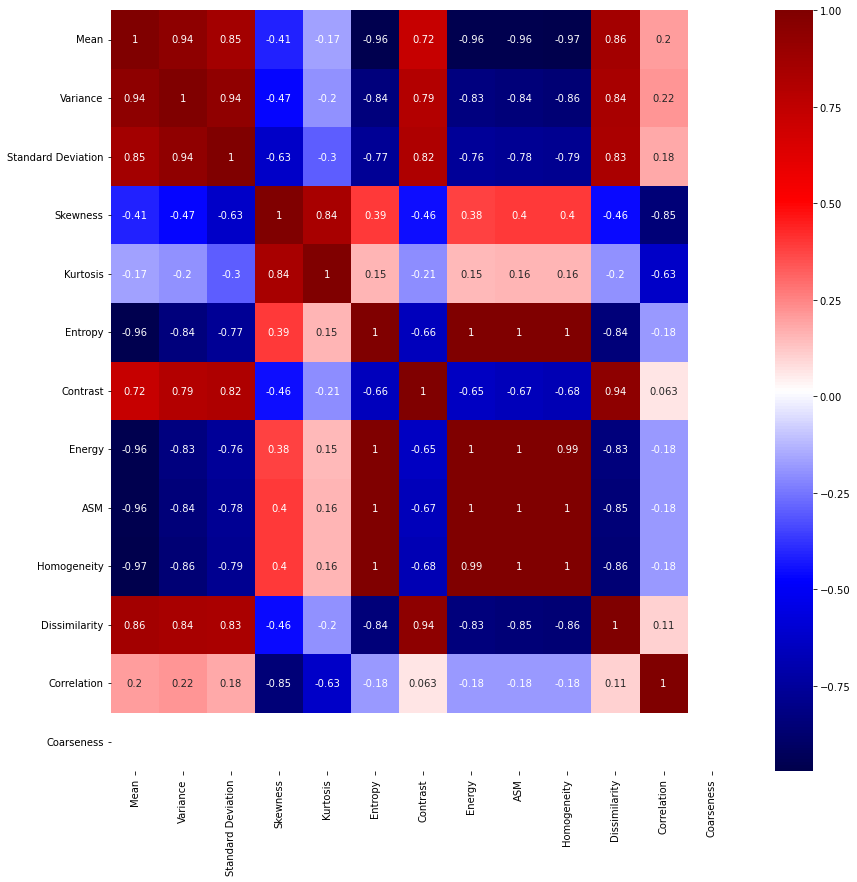
\includegraphics[width = .9\textwidth]{images/corr-matrix.png}
    \caption{Correlation Matrix}
    \label{corr-matrix}
\end{figure}

Based on this correlation plot, (figure \ref{corr-matrix})  we can begin speculating about multicollinearity. Multicollinearity is addressed in Variable Selection (section \ref{var-sel}, mainly through Elastic Net variable selection

\subsection{Histograms}
\begin{figure}[H]
    \centering
    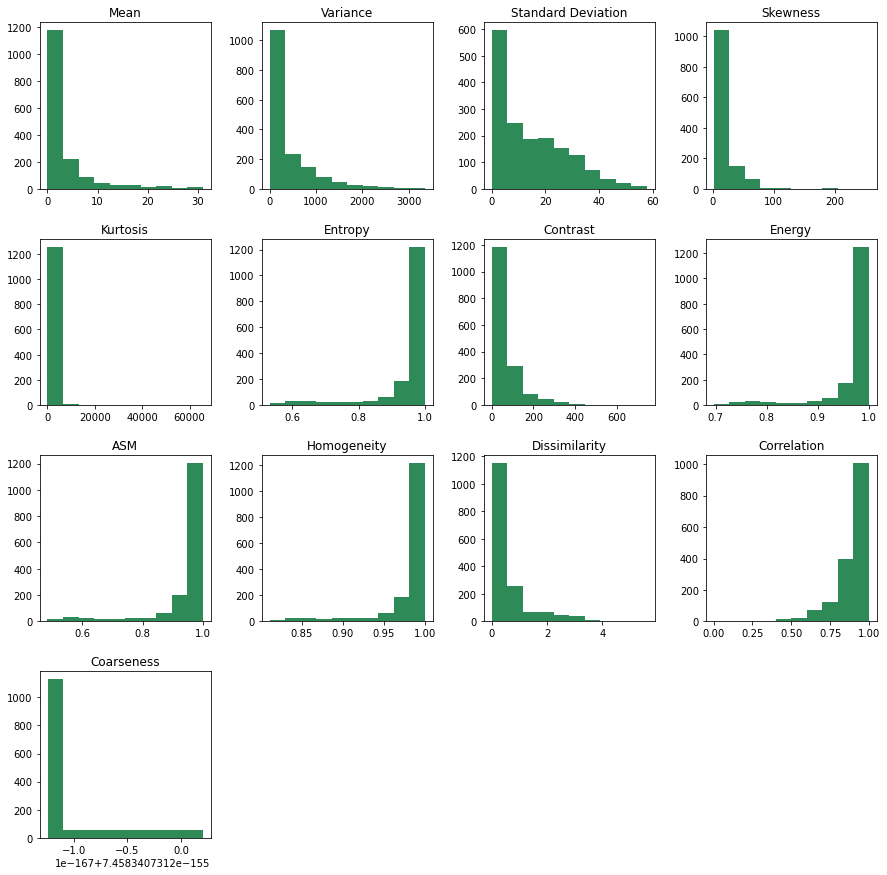
\includegraphics[width = .9\textwidth]{images/histograms.png}
    \caption{Histograms of variables}
    \label{histograms}
\end{figure}

From the histograms above (figure \ref{histograms}), we see that there may be issues with the normality assumption. All variables have large skews to the left side for variables that correspond to low types of deviation: Mean, Variance, Skewneww, etc, and to the right for variables where largest value 1 describes low deviation: Energy, Homogeneity, Entropy, etc.\\

These plots also show the difference in scales between the variables.\\

\subsection{ISOMAP}
An ISOMAP off the images using PCA shows how the images are related to one another in figure \ref{pca-image}. The image demonstrates the brain scans separated by size and darkness. While the right most portion may show tumors with the white spots in the middle, this ISOMAP is not reliable in determining if their is a tumor present or not.

\begin{figure}[H]
    \centering
    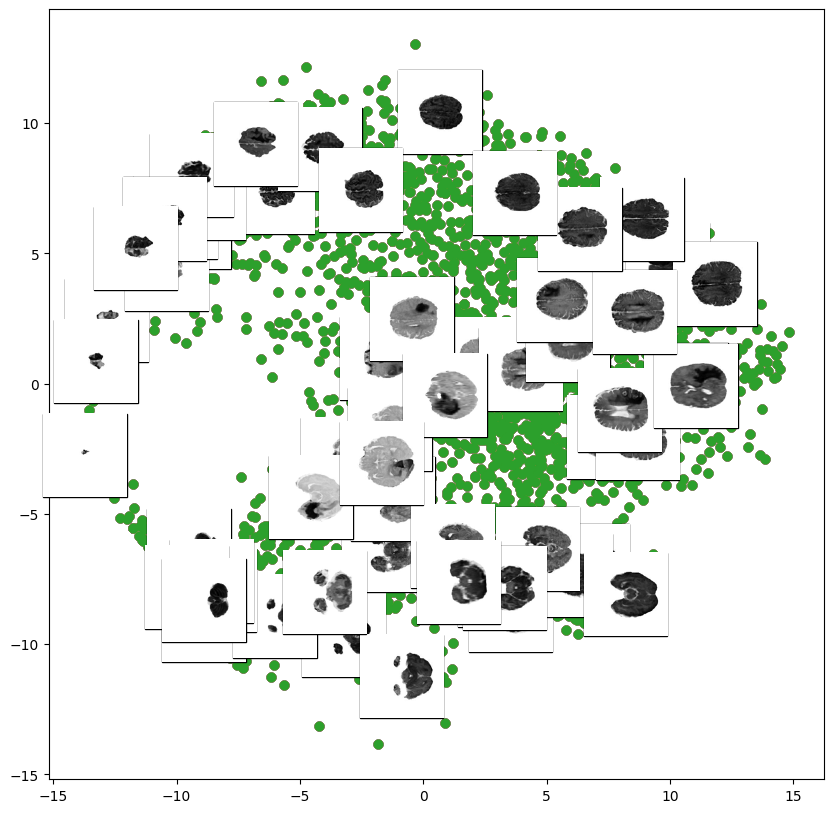
\includegraphics[width = .8\textwidth]{images/pca-image-clump.png}
    \caption{PCA Image Recognition}
    \label{pca-image}
\end{figure}

\section{Variable Selection} \label{var-sel}

Principal Components Analysis (PCA) and ElacticNet are performed to select the most important Features among the 13 first and second order Features that were extracted from the raw image files \cite{accurate-detection}. In order to objectively quantify the improvements obtained from application of these variable selection techniques, we'll begin by modeling all the variables. In addition to building models with the most important variables identified through the PCA process, we'll also build models utilizing the top four Principal Components which explain as much as 91.32\% of the variability in the data. Please note that each section name also includes that code for that variable selection that will be used in the remainder of this paper.

\subsection{Image Files (img)}
The dataset includes image files with a classification as 0: no tumor, 1: tumor. The images are reduced to 25\% of their original size and then scaled to reduce computational time. The image size reduction was especially needed for tuning and training Neural Network models, which are traditionally expensive to run.

\subsection{Raw image files with PCA (img-pca)}
The PCA on the raw image files is seen in Figure \ref{pca-image-explained}. Per the image, 10 Principal Components are selected. While this is a large number of PC's, it explains less than 80\% of the data.

\begin{figure}[H]
    \centering
    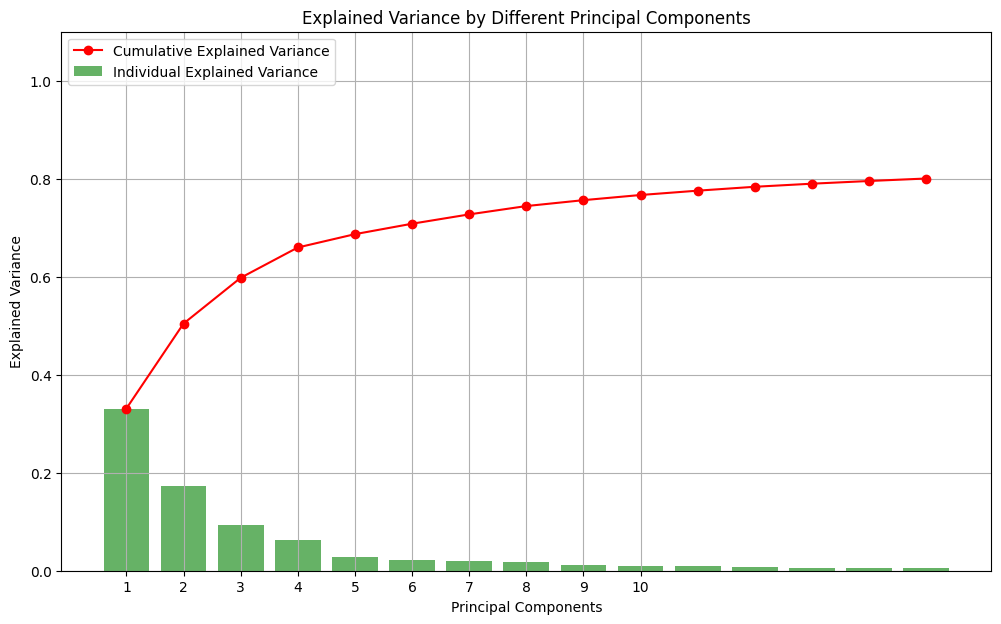
\includegraphics[width = .8\textwidth]{images/pca-images.png}
    \caption{Explained Variance in PCA on Image Dataset}
    \label{pca-image-explained}
\end{figure}

\subsection{PCA and Component Selection (pca)}

\subsection{Feature Selection with PCA (pca-select)} \label{pca-select}

The Dataset distilled to features is next considered. PCA is run on the dataset, as described in Figures \ref{feat_pca-varExp} and \ref{feat_pct-varExp}. From these images, the top four principal components are chosen to describe the dataset moving forward under this selection.

\begin{figure}[H]
    \centering
    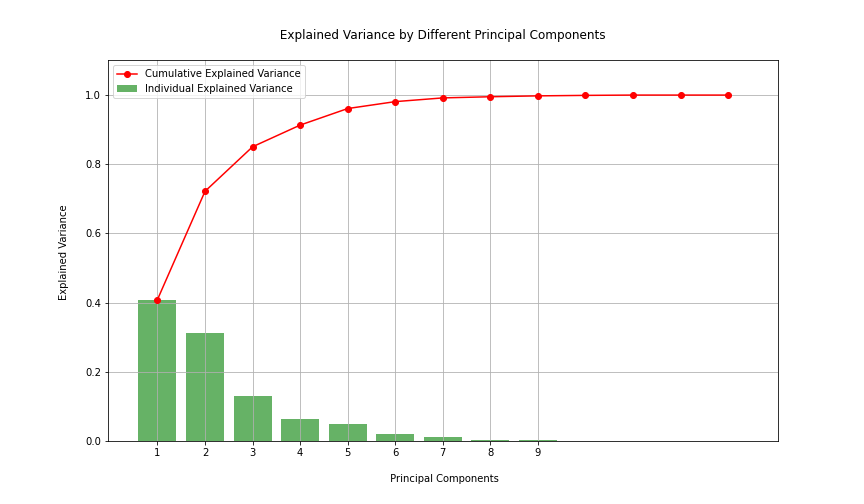
\includegraphics[width = .9\textwidth]{images/feat_var-exp.png}
    \caption{Features PCA Variance Explained}
    \label{feat_pca-varExp}
\end{figure}

\begin{figure}[H]
    \centering
    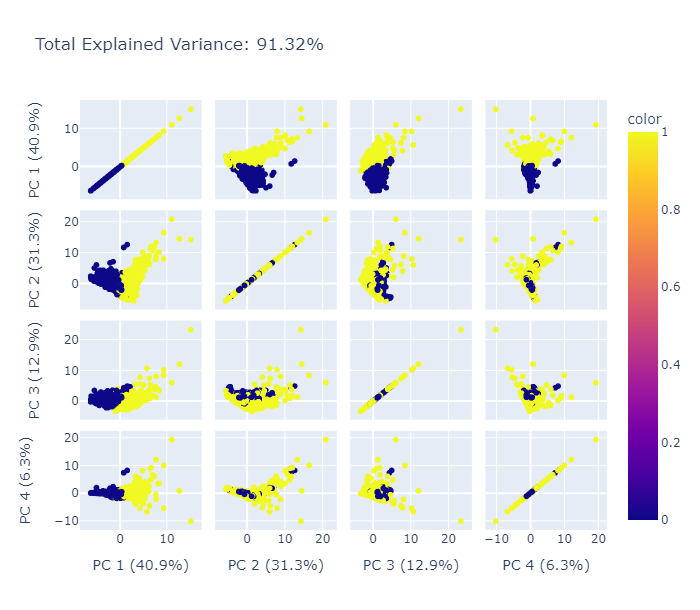
\includegraphics[width = .9\textwidth]{images/feat_perc_VarExp.png}
    \caption{Total Variance Explained by First Four Principal Components}
    \label{feat_pct-varExp}
\end{figure}

\begin{figure}[H]
    \centering
    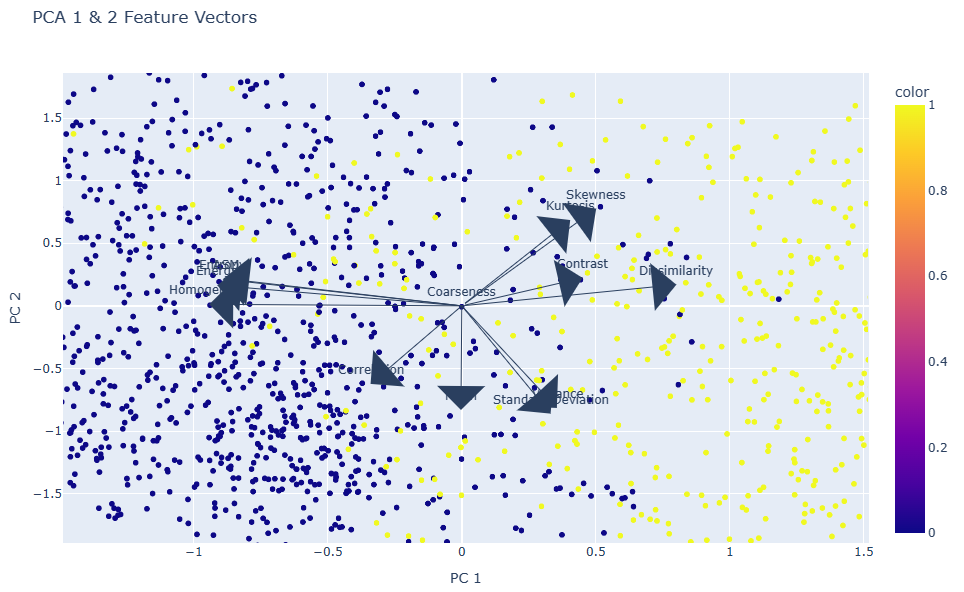
\includegraphics[width = .9\textwidth]{images/feat_vectors.png}
    \caption{Feature Vectors for the First Two Principal Components}
    \label{feat_vects-varExp}
\end{figure}

The \textbf{top four principal components} account for as much as 91.32\% of the \textbf{explained variation.}  In continuation of the Feature Dataset with PCA variable selection (section \ref{pca-select} Figure \ref{feat_vects-varExp}) displays the importance of the features by the length of their vector arrows. From this image and reading of the top features per component, the five features that will be selected for use in this analysis are: \textit{Energy, Skewness, Homogeneity, Dissimilarity, and Mean} which contribute strongly to the first four principal components in addition to the second.


\subsection{Feature Selection with Elastic Net (en-select)}

\begin{figure}[H]
    \centering
    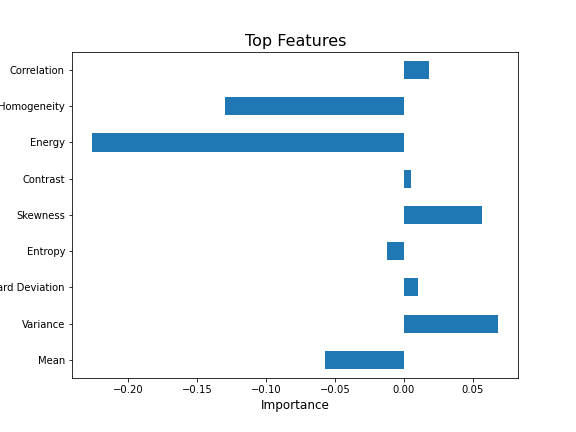
\includegraphics[width = .9\textwidth]{images/eNet_top_feats.png}
    \caption{Importance of Feature Vectors per ElasticNet}
    \label{en-feature}
\end{figure}

The last feature selection is done using Elastic Net, which was performed using the sklearn package. We tuned the penalty constant ($\alpha$) and the ElasticNet mixing ratio (l1\_ratio) using a five-fold cross validation grid search. Using ROC and AUC as the scoring mechanism, we obtained the top five variables by their importance on the final model, see in Figure \ref{en-feature}. Per this diagram, the variables chosen by this method are: \textit { Homogeneity, Energy, Skewness, Variance, and Mean}.



\section{Methodology}

The goal of this project is to find the classification model that most accurately predicts if each image contains a tumor or not. The data provided, as described in Section \ref{description-data}, are features of the images themselves, as described by Ramtekkar, Pandey, Pawar \cite{accurate-detection}. Their paper selects the five "first-order" features to describe the model, while the remaining 8 are second-order. \\

This project aims to train and tests models using these selected features, features selected by other methods, and models using the images themselves. Each model is created with the selections as described in Section \ref{var-sel}, and then split into 80/20 training and testing and cross validated 10 times to achieve the tuning results. The models are as follows:

\subsection{K-Nearest Neighbors}

 K-Nearest Neighbors is a good classification method because of its ease of use. In general, it is not computational expensive, unless applied to high dimensional data. The datasets created in Section \ref{var-sel} reduce the number of features, allowing it to avoid overfitting and high complexity with KNN. \textbf{Five-fold cross validation} was performed on the datasets to determine optimal k for each set.\\

The results of KNN after tuning for each data selection is in Table \ref{knn-tune-table}: KNN Tuning Results. Images of the tuning are in the Appendix: Table \ref{knn-tuning-picture}.

\begin{table}[H]
    \centering
    \begin{tabular}{lcrr} \toprule
       model & k & testing score & training score\\ \hline
       img & 6 & 0.9349 & 0.9435\\
       img-pca &  8 &  0.9110 &  0.9083\\
       pca & 4 & 0.9960 & 0.9791\\
       pca-select & 2 & 0.9123 & 0.9358\\
       en-select & 24 & 0.9933 & 0.9751\\
       \bottomrule
    \end{tabular}
    \caption{KNN Tuning Results}
    \label{knn-tune-table}
\end{table}

Models pca and en-select both have very high training scores, which could be due to overfitting. The testing scores for both are similarly high, though, which may suggest a good model rather than overfitting. In Results, Section \ref{sec-results}, we use the k-values shown in Table \ref{knn-tune-table}


\subsection{Support Vector Machines (SVM), Kernel and Linear}

To tune the SVM models, \textbf{Five-fold cross validation} was performed to determine the best hyperparameter for the datasets. Support Vector Machines are good models classification because of the malleable separator and ability to work with complex data. Using GridSearchCV, the models were tuned for both 'rbf' and 'linear'. All models except en-select performed better with Kernel than Linear, suggesting a non-linear model is more appropriate for this dataset. For this reason, the paper from this point on will only be using SVM-Kernel and not SVM-Linear.\\

The results are below in Table \ref{svm-table}. Almost all of the models show overfitting with the excepts of img-pca and pca-select, suggesting that PCA is near-essential before building a Support Vector Machine. The images in Table \ref{svm-tune-chart} also demonstrate overfitting as C approaches 100. There is not consistency across the models in regar to the gamma parameter.\\

GridSearchCV() did not provide the best parameters for these models; instead the visualization must be used. In SVM, the higher value C may lead to overfitting, while a smaller C creates low variance/high bias. This is evident in the images, where when C reaches 100, almost all of the accuracies are very high. The only exception is the img model, 

\begin{table}[H]
\centering
    \begin{tabular}{lrrrrrr}\toprule
    &C &gamma &kernel & testing score & training score \\\midrule
    img &100 &0.001 &rbf &0.9501 & 1 \\
    img-pca &100 &0.001 &rbf &0.9022 & 0.9365 \\
    pca &10 &0.1 &rbf &0.9741 &0.9888 \\
    pca-select &100 &0.1 &rbf &0.9567 &0.9624 \\
    en-select &10 &0.0001 &linear &0.9805 &0.9809 \\
    \bottomrule
    \end{tabular}
    \caption{Tuning Parameters for SVM} \label{svm-table}
\end{table}

Using the table above and the images in Table \ref{svm-tune-chart} in the Appendix, the optimal parameters for img, pca, and en-select are changed. The training scores in all cases are high and could indicate over fitting. The new variables are below in Table \ref{svm-table-up}.

\begin{table}[H]
\centering
    \begin{tabular}{lrrrrrr}\toprule
    &C &gamma &kernel & testing score & training score \\\midrule
    img & 1 &0.001 &rbf &0.9179 & 0.9519 \\
    img-pca &100 &0.001 &rbf &0.9022 & 0.9365 \\
    pca &10 & 0.0001 &rbf & 0.9649 & 0.9657 \\
    pca-select &100 &0.1 &rbf &0.9567 &0.9624 \\
    en-select &10 &0.0001 &rbf & 0.9589 & 0.9591 \\
    \bottomrule
    \end{tabular}
    \caption{Updated Tuning Parameters for SVM} \label{svm-table-up}
\end{table}


\subsection{Neural Networks}

Neural Networks is a good classification model that is tolerant to noisy data and flexible. \textbf{Five-fold cross validation} was performed on the datasets to determine the most effective number of hidden layers, regularization parameter, and non-linear activation function. The MLPClassifier() function from sci-kit with GridSearchCV(). The validation is performed on all 5 datasets, with the tuning results in Table \ref{nn-tune-table}. Images of tuning parameters are in Table \ref{nn-tune}\\

The table shows that the most common hidden layer size is (30, 20, 15), and the largets training school is for raw images. This combination may be a result of overfitting, over, because the mean test score is much less than that of the train score. Alternatively, with elastic net, the train and testing scores are equally high.

\begin{table}[H]
    \centering
        \begin{tabular}{lrrrrrr}\toprule
        &activation &alpha &hidden layer sizes &mean test score &mean train score \\\midrule
        img &relu &0.0001 &(40, 35) &0.9495 &0.9983 \\
        img-pca &relu &0.0778 &(40, 35, 20) &0.9063 &0.9457 \\
        pc &relu &0.0667 &(30, 20, 15) &0.9784 &0.9785 \\
        pca-select &relu &0.0334 &(30, 20, 15) &0.9412 &0.9437 \\
        en-select &relu &0.0223 &(30, 20, 15) &0.9801 &0.9814 \\
        \bottomrule
        \end{tabular}
    \caption{Neural Net Hyperparameter Tuning}
    \label{nn-tune-table}
\end{table}

\subsection{Naive Bayes}

Naive Bayes is an efficient classification method.

\subsection{Random Forest} \label{rf}

The method to produce the RandomForest Model is different from the others because the Random Forest does not require variable selection. It is robust to multicollinearity, which is seen in the dataset, and thus an appropriate choice for testing. Thus, this model is performed on the raw image dataset and full feature set.\\

GridSearchCV() was performed using \textbf{Five Fold Cross Validation} on both datasets. The parameters are below in Table \ref{rf-results}. Again, we see a model with very high mean train score and similarly high test score. Random Forest can be prone to overfitting, so the model with the highest train score is not necessarily the best. Moving forward in building the Random Forest model, \textbf{image dataset parameters: max\_depth=40, n\_estimators=200} and \textbf{feature dataset parameters: max\_depth=40, n\_estimators=200} are used for training the model.

\begin{table}[H]
    \centering
        \begin{tabular}{lllrr}
        \toprule
        & max depth & n estimators & mean test score & mean train score \\
        \midrule
        img & 8 & 200 & 0.9870 & 0.9958 \\
        features & 9 & 400 & 0.9166 & 0.9869 \\
        \bottomrule
        \end{tabular}
    \caption{Random Forest Tuning Results}
    \label{rf-results}
\end{table}

\subsection{XGBoost}

Gradient Boosting is a similarly robust model when multi-collinearity could be a problem in classification methods. Like Random Forest (sec. \ref{rf}, variable selection is not needed on the XGBoost method, and the model is performed on the raw image dataset and full feature set.\\

Because XGBoost has many parameters, RandomizedSearchCV() is a better method for choosing the parameters. All of the scores have a high train score and high test score, as was also evident in the Random Forest model. The result with highest testing score and not highest trainging score is selected. Moving forward in building the Random Forest model, \textbf{image dataset parameters: max\_depth=40, n\_estimators=200} and \textbf{feature dataset parameters: max\_depth=40, n\_estimators=200} are used for training the model.

\begin{table}[H]
    \centering
        \begin{tabular}{lrrrrrr}
        \toprule
        &subsample & max\_depth & gamma & colsample\_bytree & mean\_test\_score & mean\_train\_score \\
        \midrule
        img & 1 & 5 & 5 & 0.6 & 0.9136 & 0.9759 \\
        features &  1 & 3 & 5 & 1 & 0.9840 & 0.9884 \\
        \bottomrule
        \end{tabular}
    \caption{XGBoost Results}
    \label{tab:my_label}
\end{table}

\section{Results} \label{sec-results}

\begin{table}[H]
    \centering
        \begin{table}[H]\centering
        \renewcommand{\arraystretch}{1.15}
%        \scriptsize
        \begin{tabular}{lllrrr}\toprule
        Model &Data Type & &Accuracy &Senitivity \\\midrule
        Neural Net &Images &img &0.8924 &0.9713 \\
        & &img-pca &0.9283 &0.9045 \\
        &Extracted Features &pc &0.9920 &0.9904 \\
        & &pc-select &0.9655 &0.9427 \\
        & &en-select &0.9894 &0.9904 \\
        \hline
        SVMK &Images &img &0.9097 &0.9140 \\
        & &img-pca &0.9323 &0.9140 \\
        &Extracted Features &pc &0.9907 &0.9777 \\
        & &pc-select &0.9655 &0.9554 \\
        & &en-select &0.9841 &0.9618 \\
         \hline
        Naive Bayes &Images &img & & \\
        & &img-pca & & \\
        &Extracted Features &pc & & \\
        & &pc-select & & \\
        & &en-select &0.9562 & \\
        \hline
        KNN &Images &img &0.9349 &0.8917 \\
        & &img-pca &0.9110 &0.8471 \\
        &Extracted Features &pc &0.9960 &0.9904 \\
        & &pc-select &0.9124 &0.8185 \\
        & &en-select &0.9934 &0.9873 \\
         \hline
        Random Forest &Images & &0.9283 &0.9219 \\
        &Extracted Features & &0.9870 &0.9765 \\
        \hline
        XGBoost &Images & &0.9880 &0.9735 \\
        &Extracted Features & &0.9880 &0.9735 \\
        \bottomrule
        \end{tabular}
        \end{table}
    \caption{Metrics from All Models}
    \label{all-results}
\end{table}

The final metrics for all of the models and datasets are above in Table \ref{all-results}. The models performed differently depending on the dataset used in building and testing the model. In general, the images themselves did not perform as well as the features that came from the extracted features. While the NeuralNet  and SVM-K models returned high sensitivities for the images, the accuracies were much lower, making this not an optimal dataset, either raw or with PCA.\\

The Neural Network Model had better sensitivity results than KNN, which is important to consider as the cost of not spotting a tumor is much larger than spotting a tumor that is not there.\\ 

Amongst the selected features, the Elastic Net Method consistently performed better than the features selected through PCA. Elastic Net is used generally where multicollinearity is present, which could explain why this variable selection performed well.\\

Using the Top Four Principal Components also produced high metric for all models, especially in KNN.\\

\section{Conclusion and Findings}

In this project both the raw image files and the extracted features, performed by Ramekka, Pandey and Pawar \cite{accurate-detection}, were used. Ultimately, the extracted features in general performed better than the images themselves. The image processing performed made for a better dataset. The dataset had numerical values for the shifting in images, taking away a layer of guessing the model has to do with the raw images.\\

The high scoring of the Principal Component Selection could indicate that each feature does not contribute in a significantly independent way, thus the creation of the component can better describe the dataset. With the high performance of the Elastic Net Selection confirms, we can infer that there is high multicollinearity in this model, as presented in EDA (sec. \ref{eda}).\\

As a surprise, the CART methods did not outperform the other classification methods. Before running the models, the CART methods seemed to be the best option, as they could use all features, and, in general, are simple to run. The tuning did help with problems of overfitting. These methods may perform better on a larger dataset, so the full advantages of using Random Forest or XGBoost are not evident in this dataset.\\

Ultimately, the Neural Network Model run on the Top Four Principal Components is the best selection to explain this model. While it is computationally expensive to run, the results are consistently better than the other models.

\newpage

\section{Appendix}

\subsection{Tuning Parameters}

\footnotesize

\begin{table}[H] \label{KNN-tune}
    \centering
    \footnotesize
    \begin{tabular}{cc}

       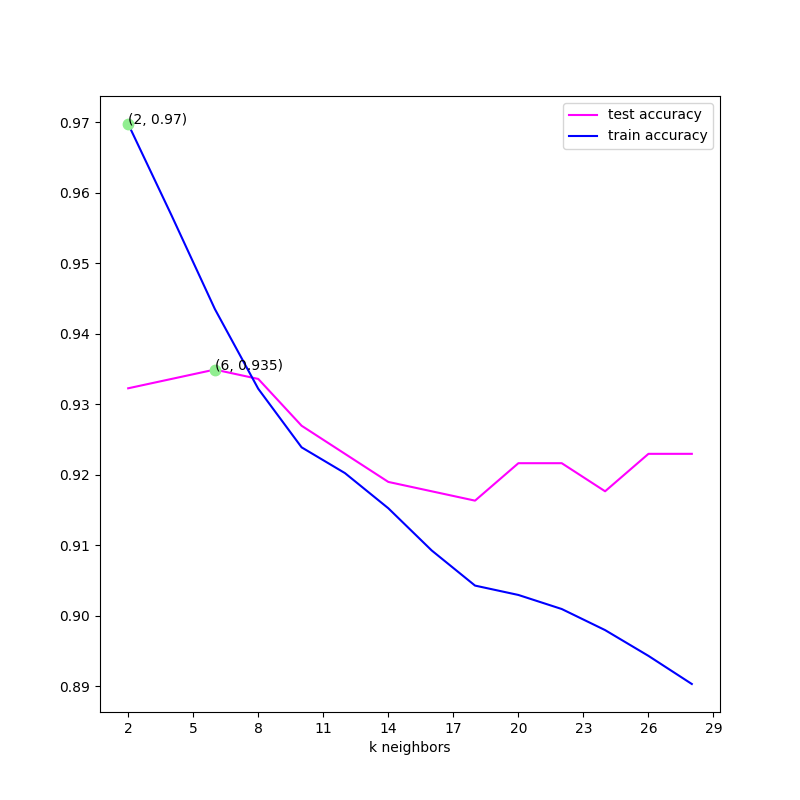
\includegraphics[width = .45\textwidth]{images/knn-tune-rawimage.png}  & 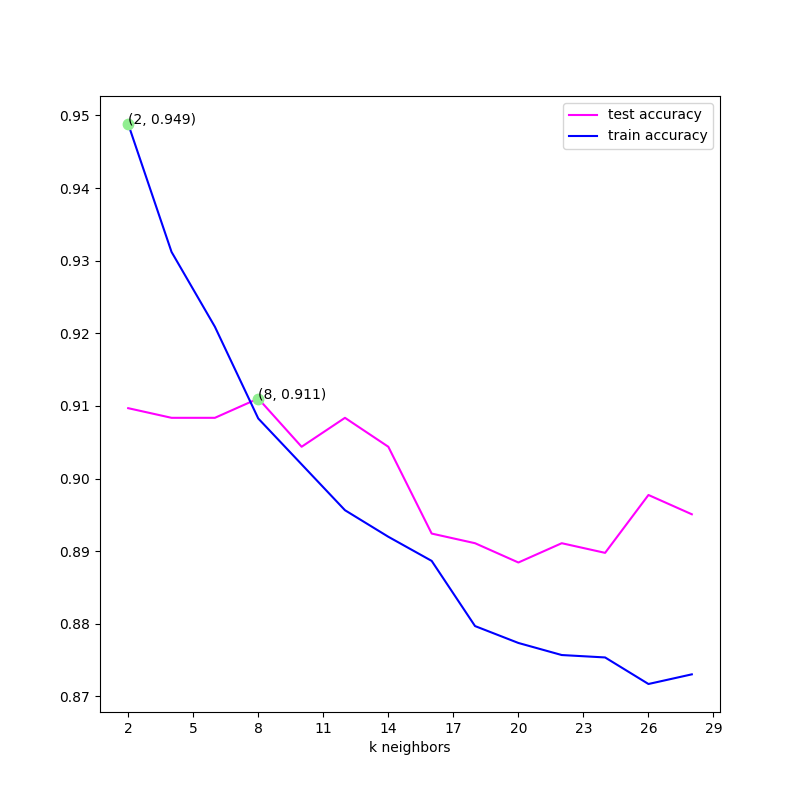
\includegraphics[width = .45\textwidth]{images/knn-tune-pcavimg.png}\\
       img  & img-pca  \\

       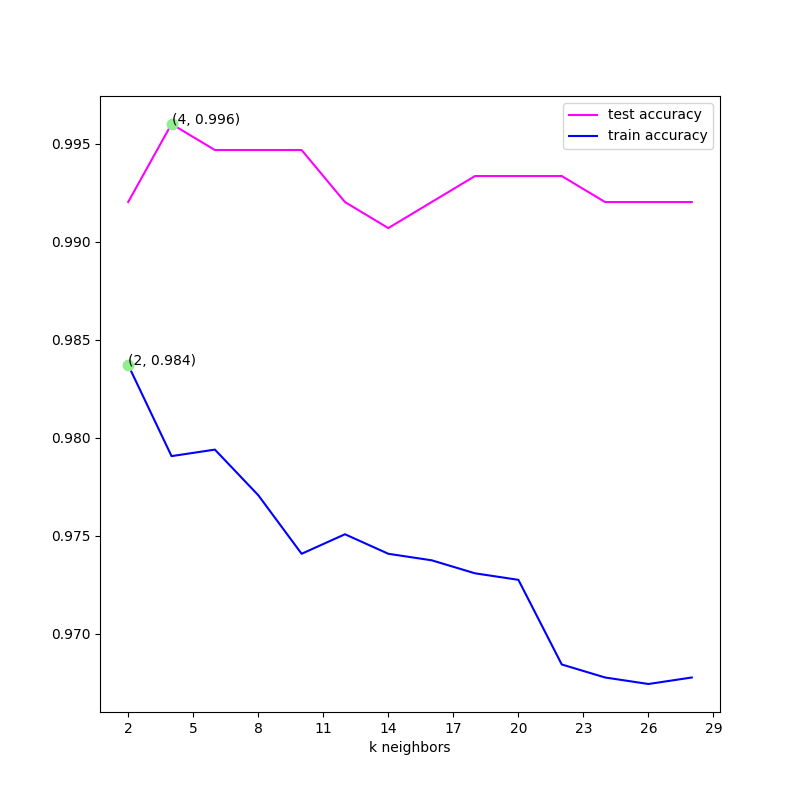
\includegraphics[width = .45\textwidth]{images/knn-tune-pc.png} & 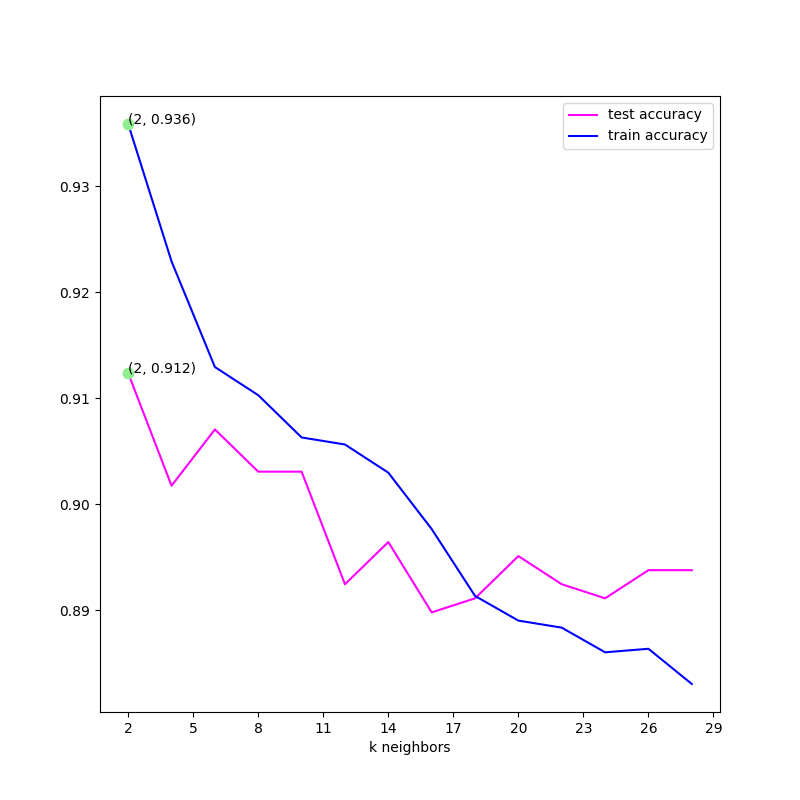
\includegraphics[width = .45\textwidth]{images/knn-tune-pcavar.png}\\
      pc& pca-select\\
       
       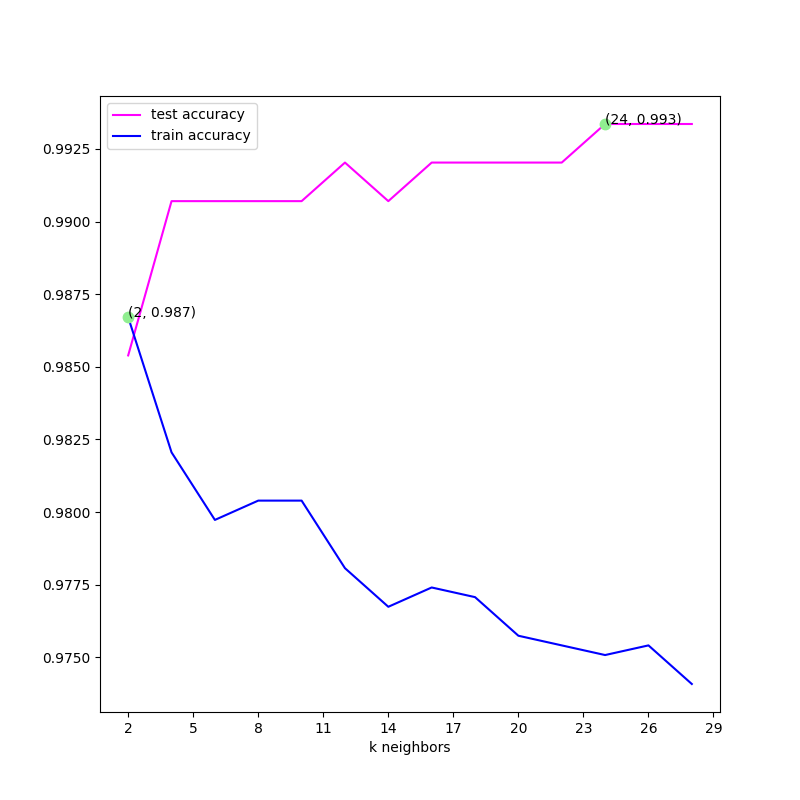
\includegraphics[width = .45\textwidth]{images/knn-tune-en.png} \\
       en-select & \\
    \end{tabular}
    \caption{KNN n\_neighbors Tuning}
    \label{knn-tuning-picture}
\end{table}

\begin{table}[H] \label{KNN-tune}
    \centering
    \footnotesize
    \begin{tabular}{cc}
       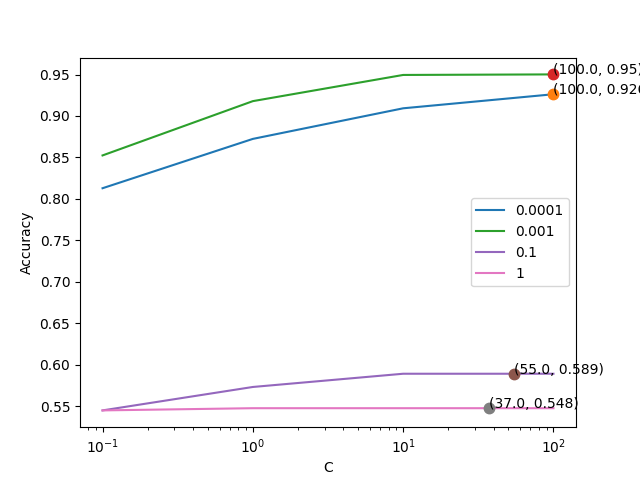
\includegraphics[width = .45\textwidth]{images/svm-tune-img.png}  & 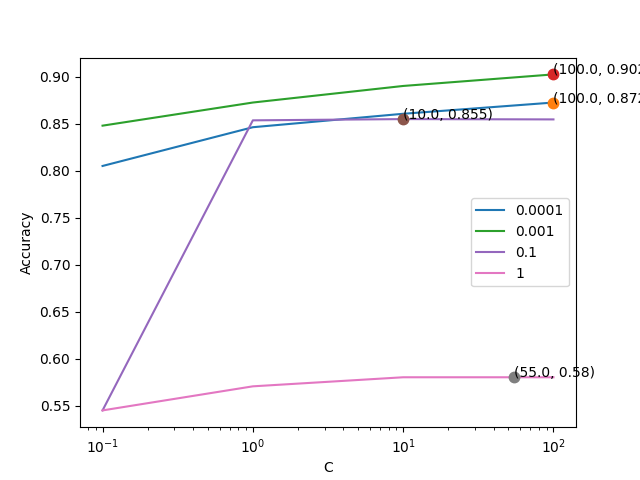
\includegraphics[width = .45\textwidth]{images/svm-tune-img-pca.png}\\
      img  & img-pca  \\
        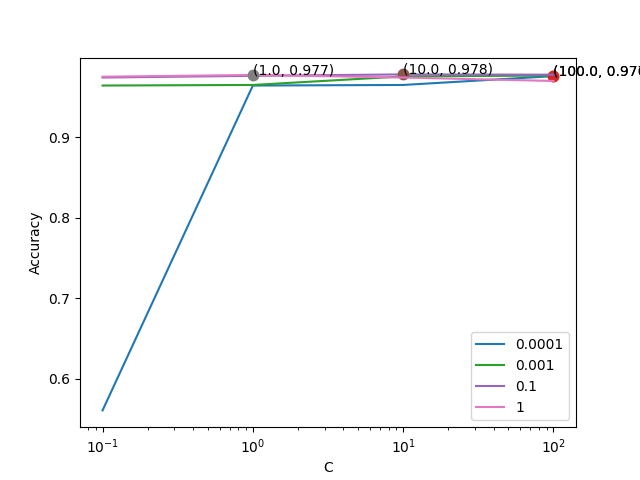
\includegraphics[width = .45\textwidth]{images/svm-tune-pc.png}  & 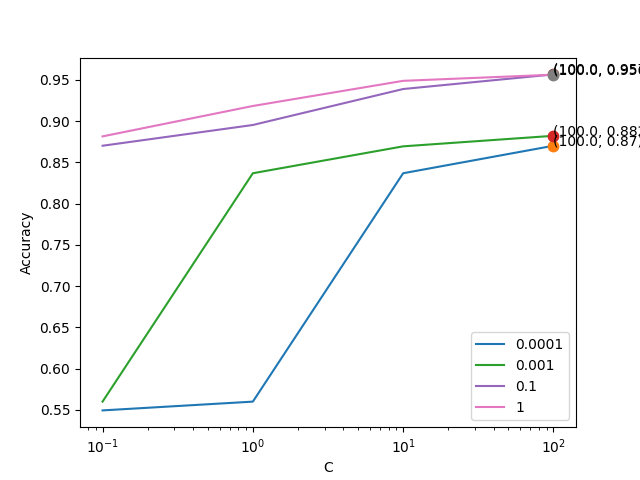
\includegraphics[width = .45\textwidth]{images/svm-tune-pca-var.png}\\
       pc& pca-select\\
       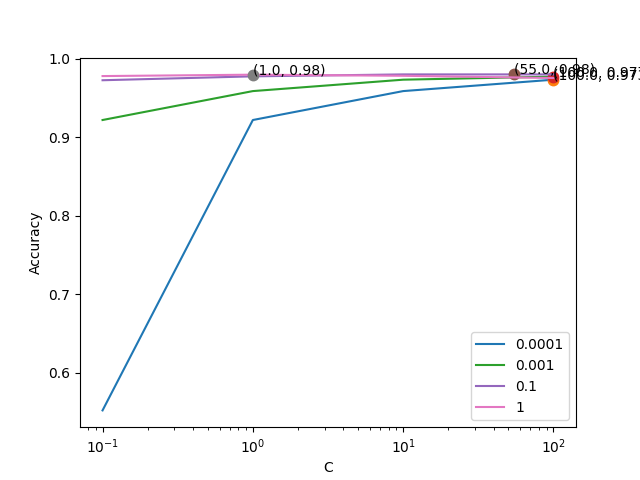
\includegraphics[width = .45\textwidth]{images/svm-tune-en-k.png} \\
         en-select & \\
    \end{tabular}
    \caption{Tuning Paramters for SVM-Kernel}
    \label{svm-tune-chart}
\end{table}

\begin{table}[H]
    \centering
    \footnotesize
    \begin{tabular}{cc}
        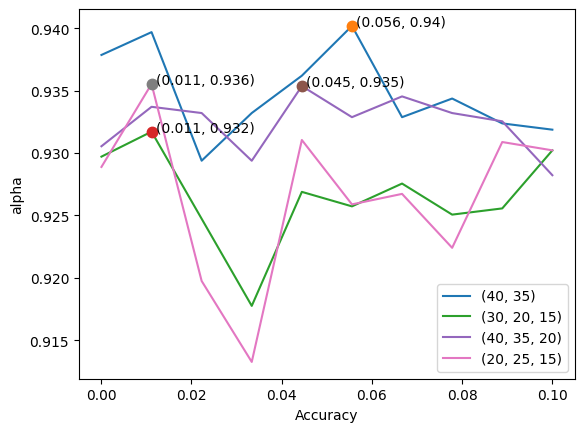
\includegraphics[width = .45\textwidth]{images/nn-tune-images.png} & 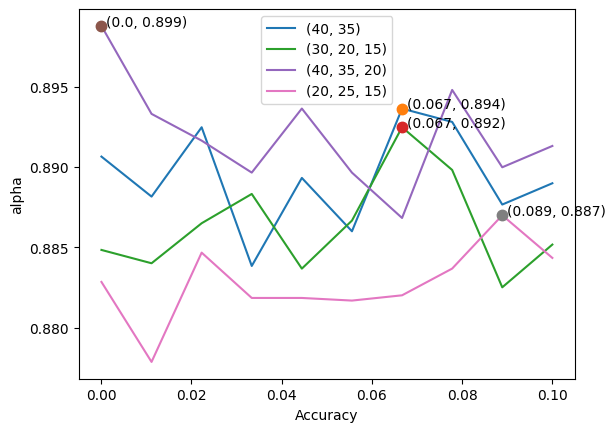
\includegraphics[width = .48\textwidth]{images/nn-tune-imagepca.png} \\
        img  &  img-pca \\
         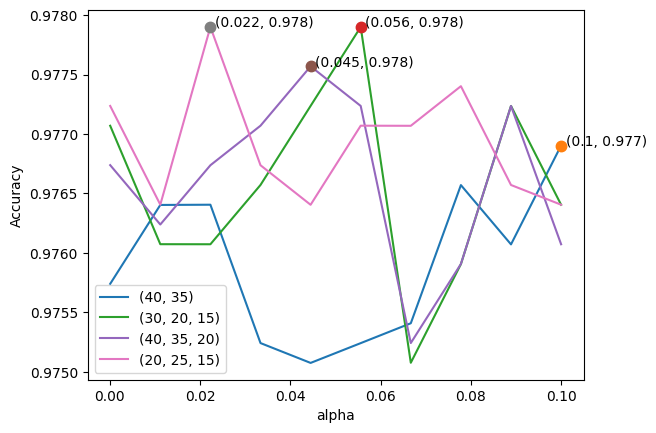
\includegraphics[width = .5\textwidth]{images/nn-tune-pca4.png}& 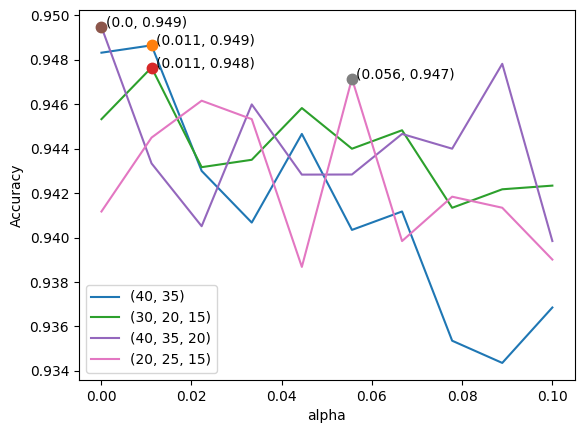
\includegraphics[width = .45\textwidth]{images/nn-tune-pcavar.png}\\
         pc & pca-select \\
         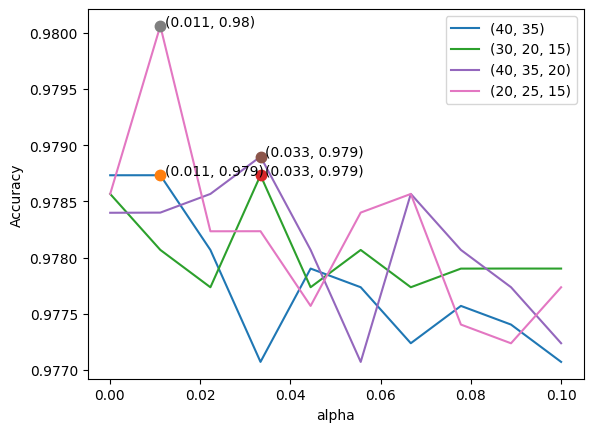
\includegraphics[width = .45\textwidth]{images/nn-tune-en.png} &\\
         en-select & 
    \end{tabular}
    \caption{Neural Net Hyperparameter Tuning}
    \label{nn-tune}
\end{table}


\subsection{Confusion Matrices}

\begin{multicols}{2}
\footnotesize
% KNN
\begin{figure}[H]
    \centering
    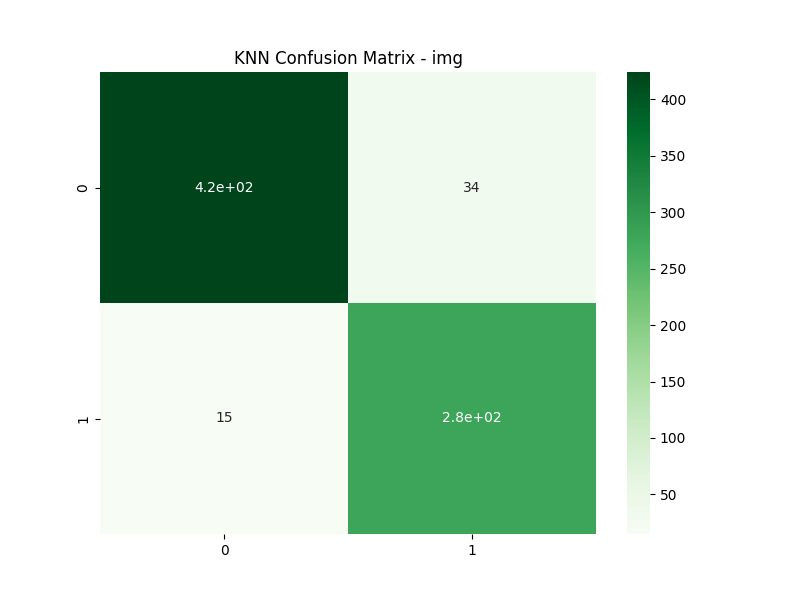
\includegraphics[width = .48\textwidth]{confusion/knn-confusion-img.png}
    \caption{KNN Confusion Matrix - img}
    \label{fig:enter-label}
\end{figure}

\begin{figure}[H]
    \centering
    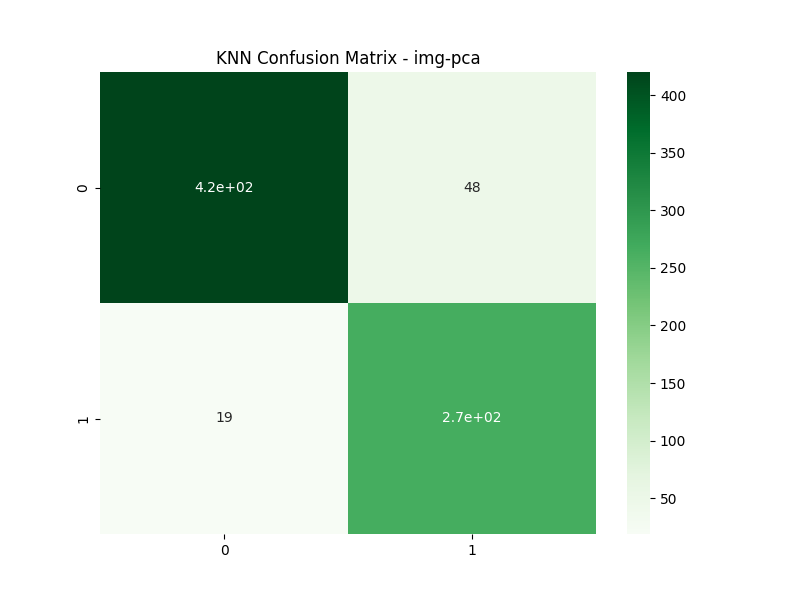
\includegraphics[width = .48\textwidth]{confusion/knn-confusion-img-pca.png}
    \caption{KNN Confusion Matrix - img-pca}
    \label{fig:enter-label}
\end{figure}

\begin{figure}[H]
    \centering
    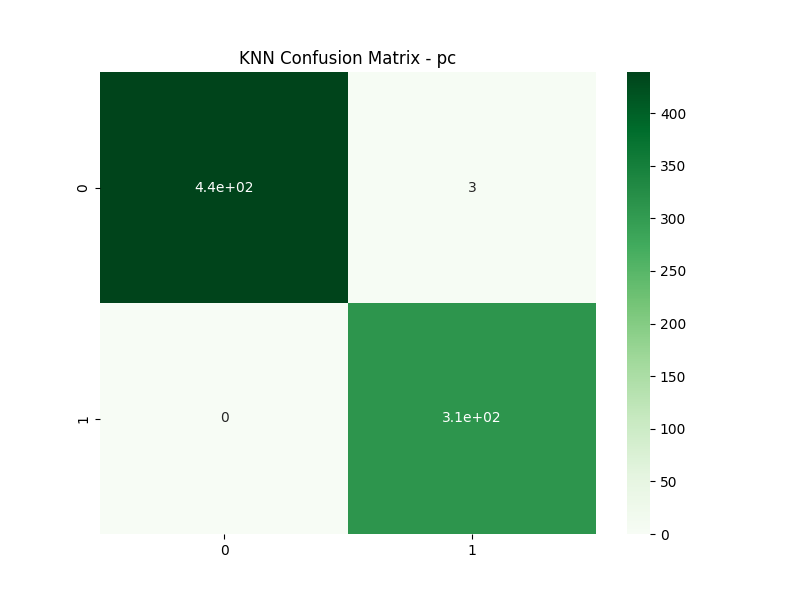
\includegraphics[width = .48\textwidth]{confusion/knn-confusion-pc.png}
    \caption{KNN Confusion Matrix - pc}
    \label{fig:enter-label}
\end{figure}

\begin{figure}[H]
    \centering
    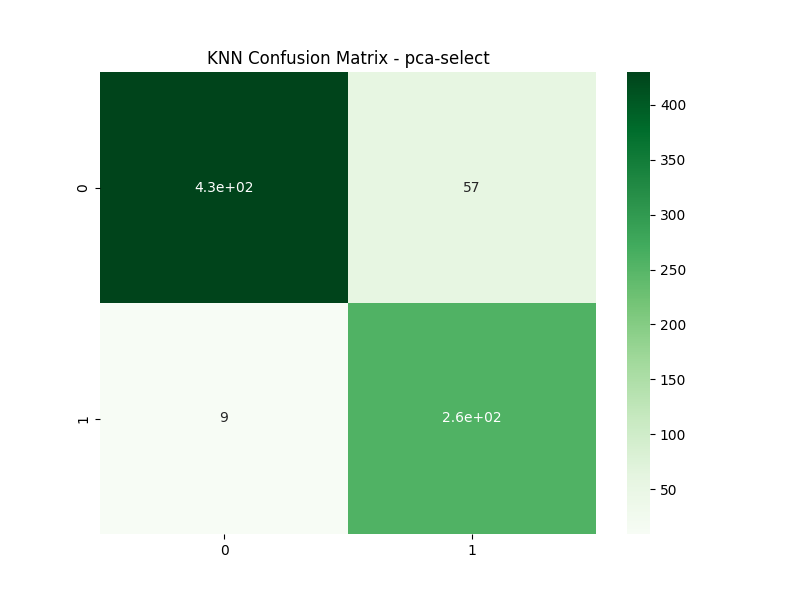
\includegraphics[width = .48\textwidth]{confusion/knn-confusion-pca-select.png}
    \caption{KNN Confusion Matrix - pca-select}
    \label{fig:enter-label}
\end{figure}

\begin{figure}[H]
    \centering
    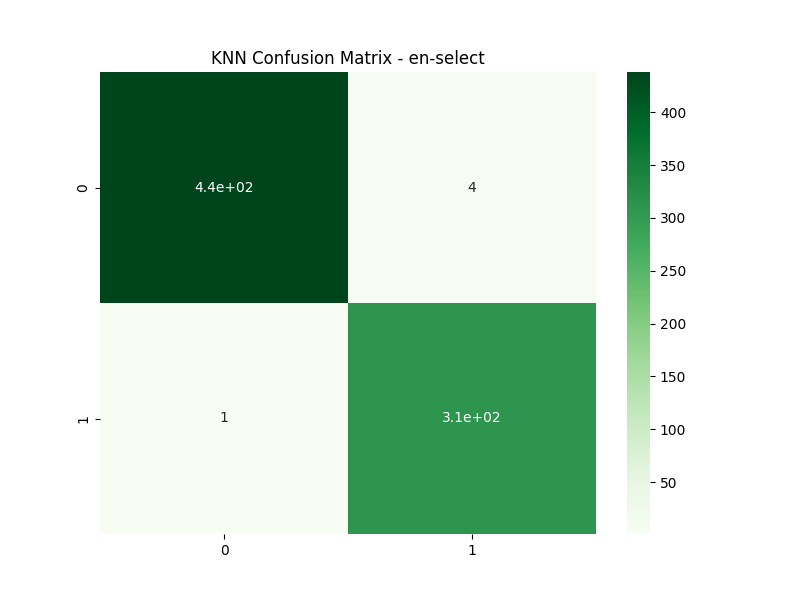
\includegraphics[width = .48\textwidth]{confusion/knn-confusion-en-select.png}
    \caption{KNN Confusion Matrix - en-select}
    \label{fig:enter-label}
\end{figure}

% SVMK
\begin{figure}[H]
    \centering
    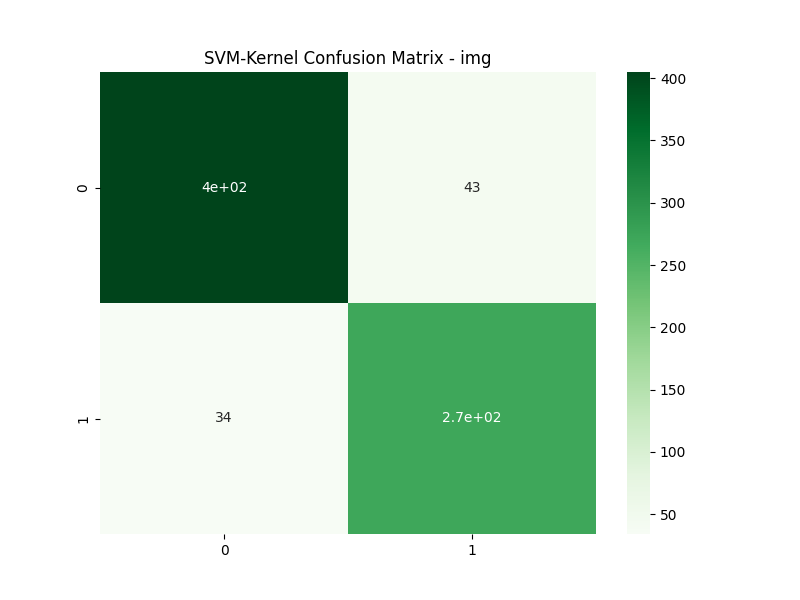
\includegraphics[width = .48\textwidth]{confusion/svmK-confusion-img.png}
    \caption{SVM-K Confusion Matrix - img}
    \label{fig:enter-label}
\end{figure}

\begin{figure}[H]
    \centering
    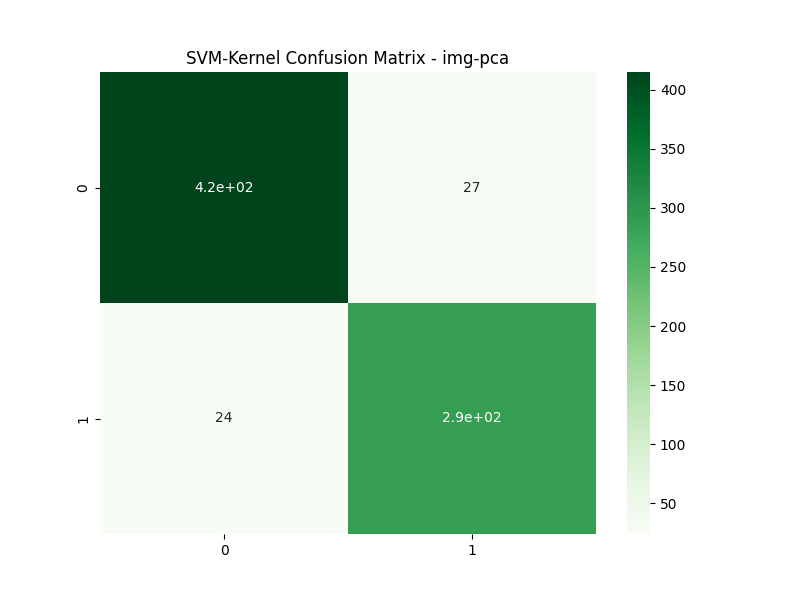
\includegraphics[width = .48\textwidth]{confusion/svmK-confusion-img-pca.png}
    \caption{SVM-K Confusion Matrix - img-pca}
    \label{fig:enter-label}
\end{figure}

\begin{figure}[H]
    \centering
    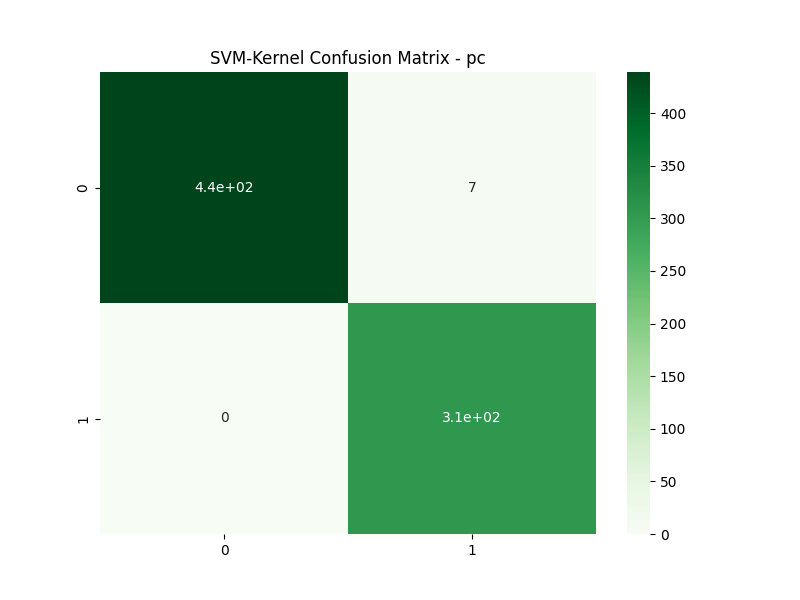
\includegraphics[width = .48\textwidth]{confusion/svmK-confusion-pc.png}
    \caption{SVM-K Confusion Matrix - pc}
    \label{fig:enter-label}
\end{figure}

\begin{figure}[H]
    \centering
    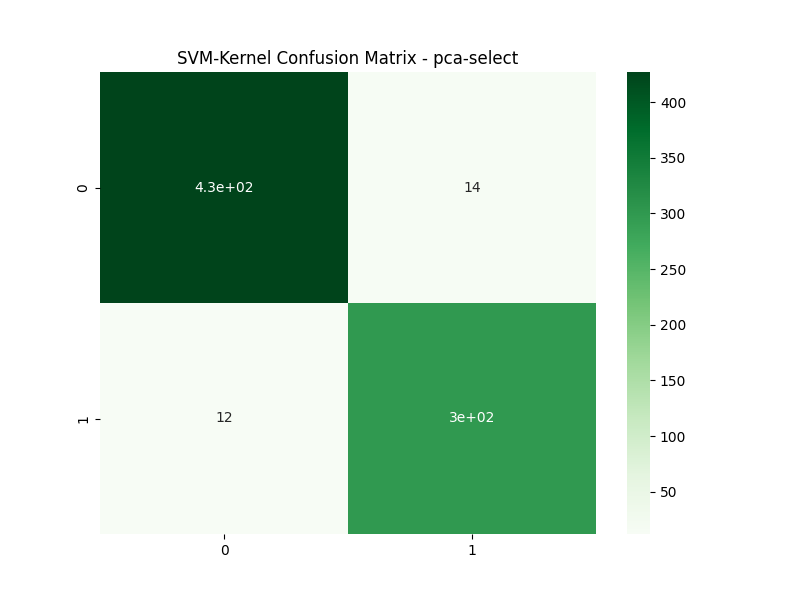
\includegraphics[width = .48\textwidth]{confusion/svmK-confusion-pca-select.png}
    \caption{SVM-K Confusion Matrix - pca-select}
    \label{fig:enter-label}
\end{figure}

\begin{figure}[H]
    \centering
    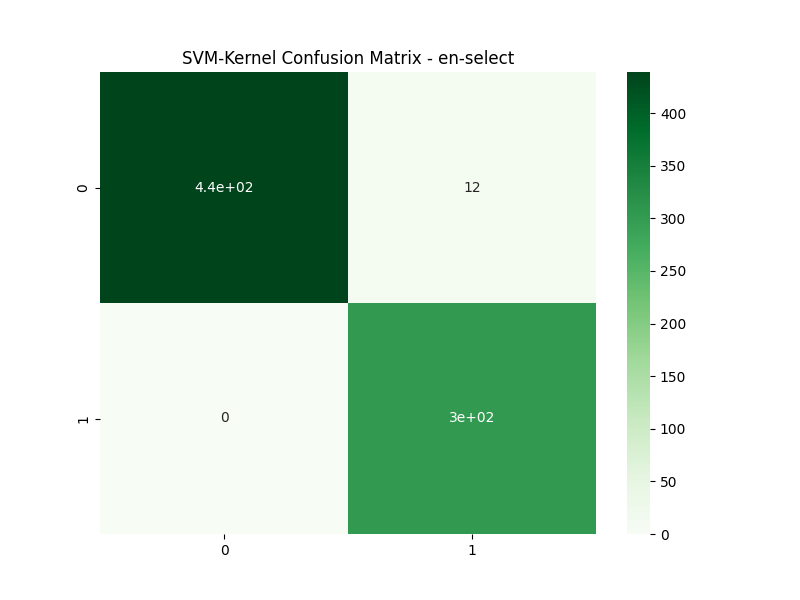
\includegraphics[width = .48\textwidth]{confusion/svmK-confusion-en-select.png}
    \caption{SVM-K Confusion Matrix - en-select}
    \label{fig:enter-label}
\end{figure}

%NEURAL NET
\begin{figure}[H]
    \centering
    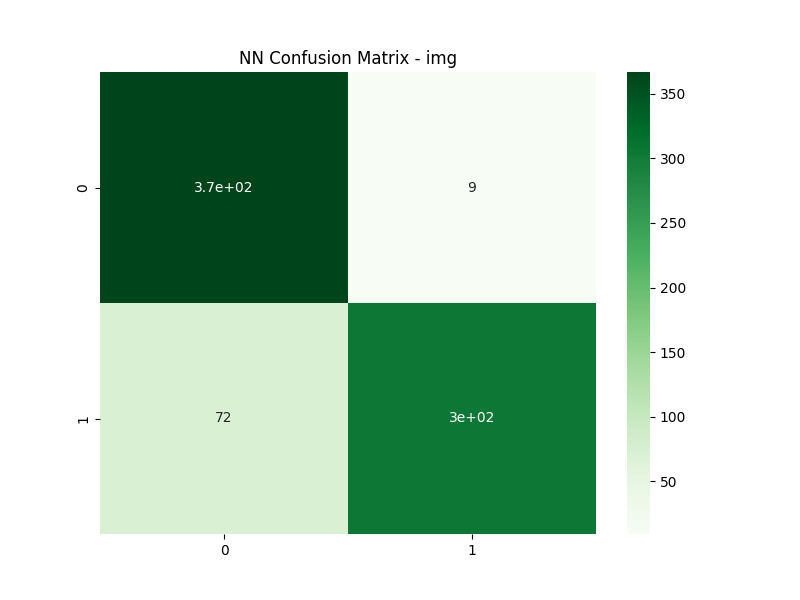
\includegraphics[width = .48\textwidth]{confusion/nn-confusion-img.png}
    \caption{Neural Net Confusion Matrix - img}
    \label{fig:enter-label}
\end{figure}

\begin{figure}[H]
    \centering
    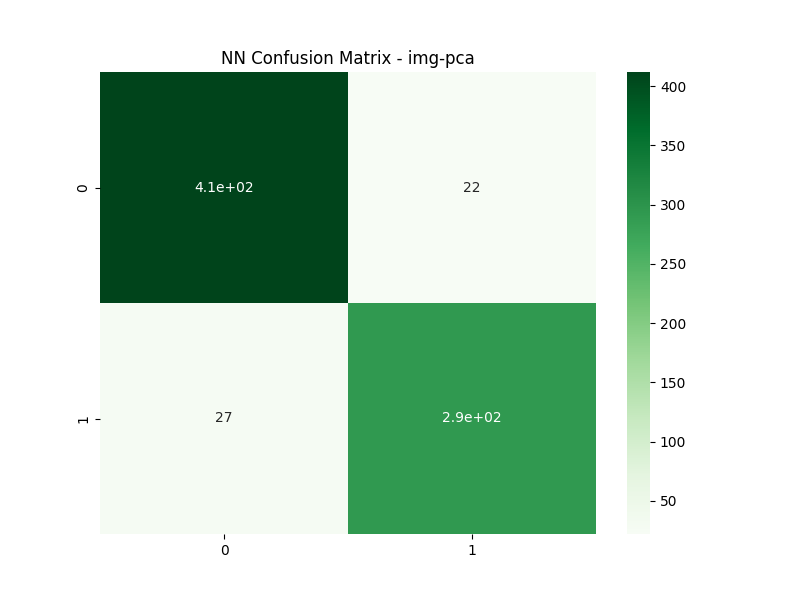
\includegraphics[width = .48\textwidth]{confusion/nn-confusion-img-pca.png}
    \caption{Neural Net Confusion Matrix - img-pca}
    \label{fig:enter-label}
\end{figure}

\begin{figure}[H]
    \centering
    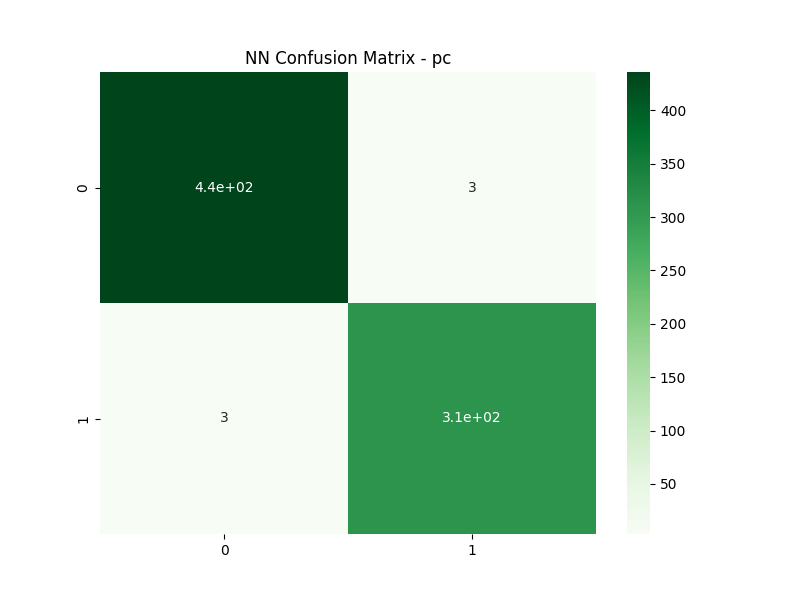
\includegraphics[width = .48\textwidth]{confusion/nn-confusion-pc.png}
    \caption{Neural Net Confusion Matrix - pc}
    \label{fig:enter-label}
\end{figure}


\begin{figure}[H]
    \centering
    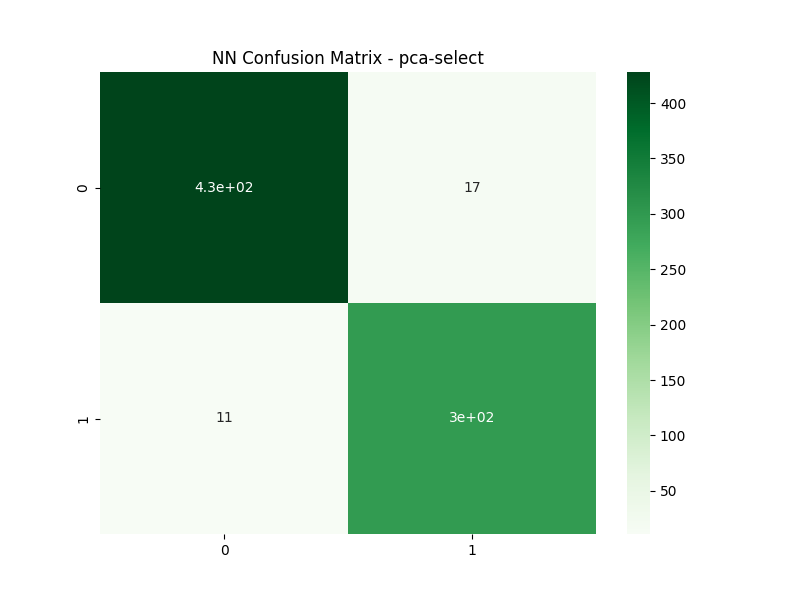
\includegraphics[width = .48\textwidth]{confusion/nn-confusion-pca-select.png}
    \caption{Neural Net Confusion Matrix - pca-select}
    \label{fig:enter-label}
\end{figure}

\begin{figure}[H]
    \centering
    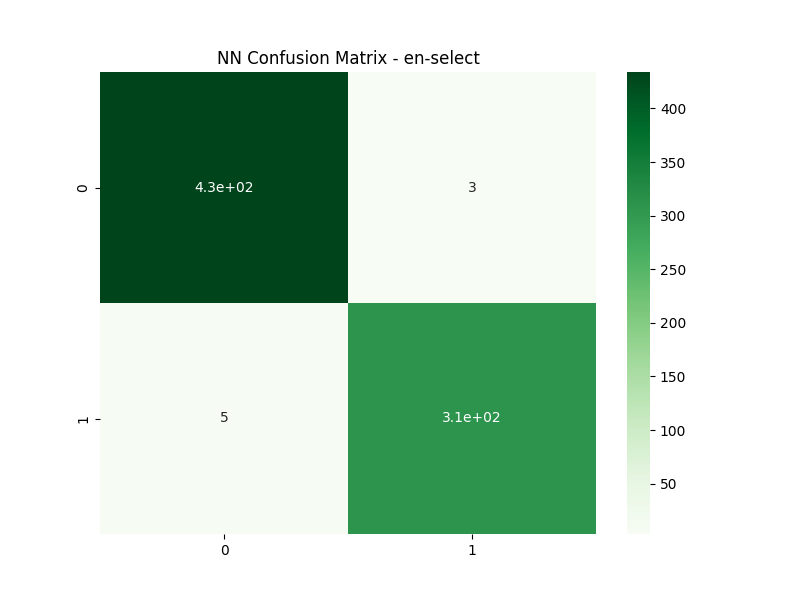
\includegraphics[width = .48\textwidth]{confusion/nn-confusion-en-select.png}
    \caption{Neural Net Confusion Matrix - en-select}
    \label{fig:enter-label}
\end{figure}

\begin{figure}[H]
    \centering
    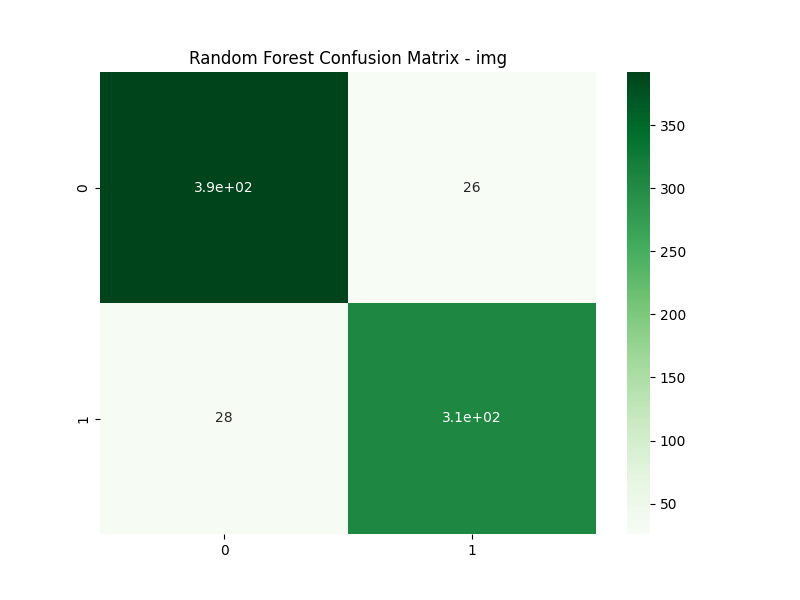
\includegraphics[width = .48\textwidth]{confusion/RF-confusion-img.png}
    \caption{Random Forest Confusion Matrix - img}
    \label{fig:enter-label}
\end{figure}

\begin{figure}[H]
    \centering
    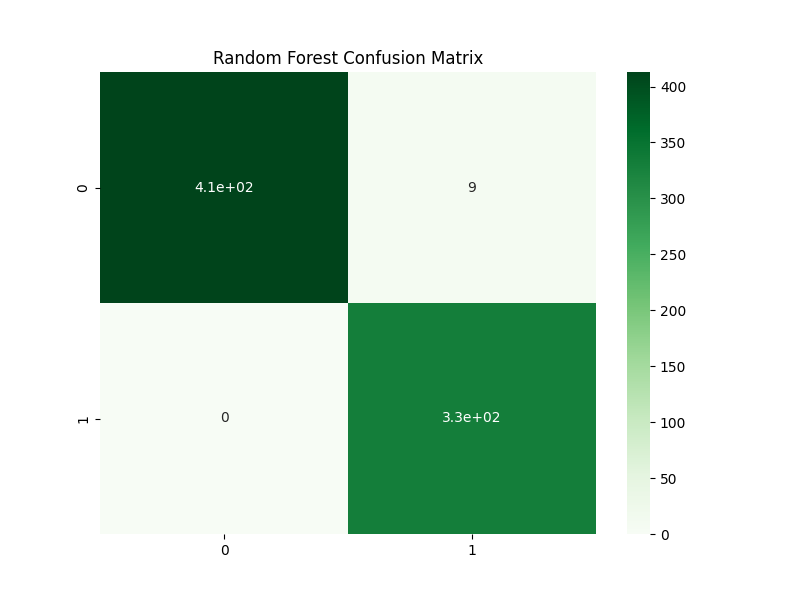
\includegraphics[width = .48\textwidth]{confusion/RF-confusion.png}
    \caption{Random Forest Confusion Matrix}
    \label{fig:enter-label}
\end{figure}

\begin{figure}[H]
    \centering
    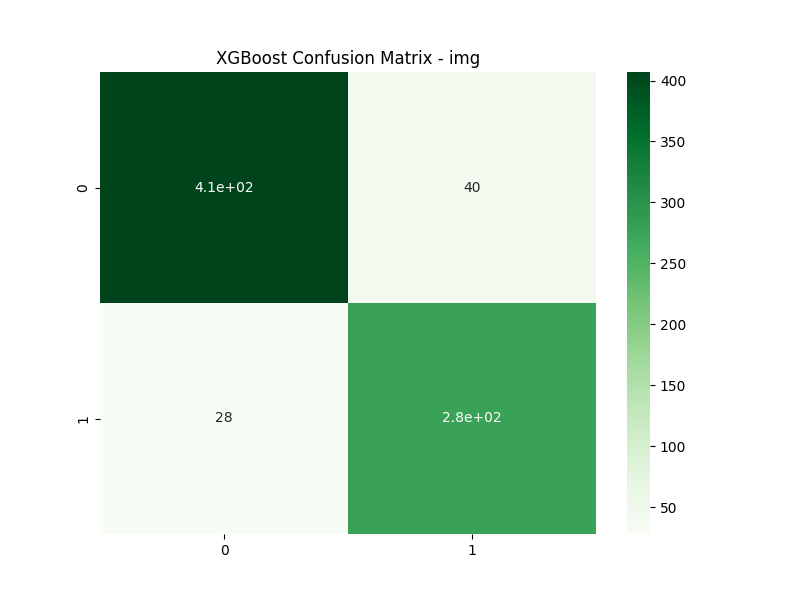
\includegraphics[width = .48\textwidth]{confusion/xgb-confusion-img.png}
    \caption{Random Forest Confusion Matrix - img}
    \label{fig:enter-label}
\end{figure}

\begin{figure}[H]
    \centering
    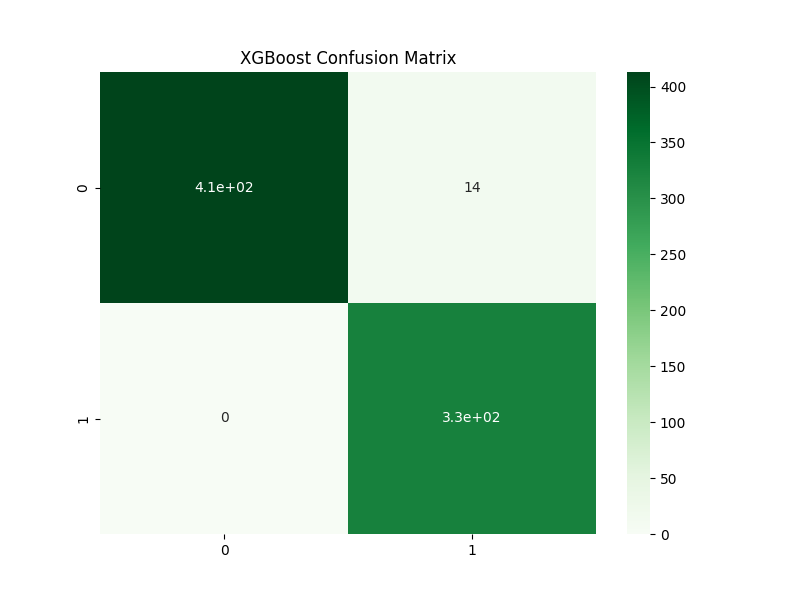
\includegraphics[width = .48\textwidth]{confusion/xgb-confusion.png}
    \caption{Random Forest Confusion Matrix}
    \label{fig:enter-label}
\end{figure}

\end{multicols}



\bibliographystyle{alpha}
\bibliography{sample}

\end{document}
